\documentclass[11pt]{article}

\usepackage{microtype}
\usepackage{amsmath}
\usepackage{float}
\usepackage[colorlinks, urlcolor = blue]{hyperref}

\usepackage{graphicx}
\usepackage{caption}
\usepackage{subcaption}

\title{\textbf{Fast Depth Map Estimation from Stereo Camera Systems}\\Project Documentation SLAM For UAV's}
\author{Malik Al-hallak 90020\\
		Hagen Hiller 110514 }
\date{Winter term 2014/15}
\begin{document}

\maketitle

%\renewcommand\thesubsection{\alph{subsection}.}

\abstract{The major goal of the project \emph{SLAM For UAV's} is to implement a SLAM algorithm on an \emph {\href{http://www.asctec.de/en/uav-uas-drone-products/asctec-pelican/}{AscTec Pelican}}. Since this goal covers several topics, we split the project group and work on different subtopics. In this documentation we describe how a stereo camera system is used to create depth maps, which then can be used for further tasks like obstacle avoidance or 3D reconstruction. We will describe the complete pipe line, from stereo camera images to a depth map and the tools needed.}

\section{Introduction}
\section{Related Work}
\section{System Description}
In this section we will describe the developed system in detail. First we will give an overview of computing depth maps in general. Furthermore,we will list the dependencies of the system. Next we will explain the developed framework and how the single components work with each other.

Although we will outline the pipeline of generating a depth image from a stereo system, we expect the reader to inform oneself about single steps and conventional knowledge in computer vision.

\subsection{Depth Map Estimation 101}\label{sec:101}
In this section we will give a rough introduction on how one can generate depth maps from a stereo camera system. This process is organised in three main steps:
\begin{itemize}
	\item image preprocessing
	\item similarity measurement
	\item 3D-coordinate calculation
\end{itemize}
\subsubsection{Image Preprocessing} %TODO un/distortete/rectified Bilder aufnehmen
The preprocessing step is done on two levels; one is the single camera and the second is the stereo system. Each image has some distortions due to the camera's lens. This distortions need to be corrected for the further steps. With the help of a calibration pattern we can calibrate the cameras. This will detect and correct distortions. The process is called \emph{undistortion}

During the process of depth map estimation we are going to take features in the left image and search them in the right image. But since this is a 2D search domain ($x$ and $y$ direction) it would be nice to ensure that the searched feature in the right image is at least in the same row as in the left image. This process is called \emph{rectification}. After the rectification step, we can assume that the cameras have no horizontal shift anymore. This reduces the feature search problem to a one dimensional (vertical) search problem. Furthermore, under the precondition that there is only a vertical shift and both cameras are identical, we can say that a feature from column $x_{Left}$ is at least at the same position in the right image so it holds that $x_{Right}\geq x_{Left}$. This also reduces the search problem, since the closer $x_{Left}$ is to $x_{Max}$ the smaller is the set of elements to search.

\subsubsection{Similarity Measure}
At this step we assume that we have undistorted and rectified images. Now we compare the left and right images. If the horizontal shift of an object from the left to the right image is large, the object is near the cameras. If the horizontal shift moves towards zero, the object is far away from the origin (the cameras).

But how can one determine the horizontal shift of an object? There exist plenty possibilities to do this. We tried three different approaches: template matching with different similarity measures, block matching and semi-global block matching. The result of each is a map with integers. The map has the same size as the two images and contains for each pixel $p(x,y)$ a value (the disparity) which expresses the horizontal shift in pixels from the left to the right image. In our framework we use the semi-global block matching (SGBM) since it has the best tradeoff between time and accuracy. The block matching mechanism is a little bit faster but very noisy at the moment. The template matching strategy takes far to long to evaluate a single picture pair. 

The SGBM tries to minimize a global energy function through different paths to the current pixel. Please have a look on \cite{hirschmuller2005accurate} and \cite{hirschmuller2008stereo} for further reading on the semi global matching. The SGBM extends the explained semi-global matching to a faster semi-global block matching.

Furthermore the SGBM guarantees smooth disparity maps with closed shapes. Figure \ref{fig:ex1_sgbm} shows the input and the result of the SGBM disparity calculation.

\begin{figure}[H]
        \centering
        \begin{subfigure}[b]{0.45\textwidth}
                \includegraphics[width=\textwidth]{images/ex1_left}
                \caption{The recitified left image}
                \label{fig:ex1_left}
        \end{subfigure}\hfill  
        \begin{subfigure}[b]{0.45\textwidth}
                \includegraphics[width=\textwidth]{images/ex1_right}
                \caption{The rectified right Image}
                \label{fig:ex1_right}
        \end{subfigure}

        \begin{subfigure}[b]{\textwidth}
                \includegraphics[width=\textwidth]{images/ex1_sgbm_norm}
                \caption{The calculated disparity map using the SGBM}
                \label{fig:ex1_sgbm_norm}
        \end{subfigure}
        \caption{Disparity calculation using SGBM}\label{fig:ex1_sgbm}
\end{figure}

\subsubsection{3D-Coordinate Calculation}
The last step is the reprojection from the image plane to the real world. We therefore use the reprojection matrix $Q$, which is constructed as follows:

\begin{figure}[H]
\centering
\begin{align*}
Q=
\begin{pmatrix}
1 & 0 & 0 & -C_{x\;left} \\
0 & 1 & 0 & -C_{y} \\
0 & 0 & 0 & f_x \\
0 & 0 & -\frac{1}{T_x} & \frac{C_{x\;right}-C_{x\;left}}{T_x}
\end{pmatrix}
\end{align*}
\captionsetup{justification=justified,margin=1cm}
\caption*{
 $C_{x\;left}$ -- x coordinate of the principal point of the left camera\\
 $C_{x\;right}$ -- x coordinate of the principal point of the right camera\\
 $C_{y}$ -- y coordinate of the principal point in both cameras\\
 $f_x$ -- focal length in x direction of the rectified image\\
 $T_x$ -- the baseline}
\end{figure}



So to reproject a point to 3D coordinates we need the $x$ and $y$ position in the left image, the disparity value $d(x,y)$ and $Q$. We construct a vector $\vec{o}=(x\;y\;d\;1)^T$ and multiply $Q$ with it so we obtain 3D coordinates $\vec{c}=(X\;Y\;Z\;W)$ which we have to divide by $W$.

\begin{align*}
	\vec{c}&=Q\cdot \vec{o}\;^T = (X\;Y\;Z\;W)^T\\
	\frac{\vec{c}}{W}&=\left(\frac{X}{W}\;\frac{Y}{W}\;\frac{Z}{W}\;1\right)^T
\end{align*}

This can be done with every pixel $(x,y)$ which has a valid disparity value $d$. It is possible to determine the coordinates of single points, e.g. for obstacle avoidance, or to produce point clouds from the images, e.g. for 3D reconstruction tasks.


\bigskip This three steps form the rough pipe line to generate depth maps from stereo camera systems. In the further sections we will explain the developed framework.

\subsection{Hardware and Dependencies}  
The AscTec Pelican is equipped with two  \emph{\href{http://www.matrix-vision.com/USB2.0-single-board-camera-mvbluefox-mlc.html?camera=mvBlueFOX-MLC200wC&selectInterface=Alle&selectMpixels=Alle&selectFps=Alle&selectSensor=Alle&selectColor=Alle&selectSize=Alle&selectShutter=Alle&selectModel=Alle&col=1&row=0}{mvBlueFOX -- MLC 200w}} cameras from \emph{\href{http://www.matrix-vision.com/home-en.html}{Matrix Vision}}. To use the cameras one need to download and install the \href{http://www.matrix-vision.com/programming-interface-mvimpact-acquire.html}{mvIMPACT Acquire SDK}. This SDK comes with the required drivers and a API for several programming languages such as C/C++, C\# etc. 

The system uses the SDK just for image acquisition, either in full resolution (752x480) or in binning mode with half resolution (376x240).

After the images are acquired they are transferred to OpenCV matrices. Therefore, \href{http://opencv.org/}{OpenCV} is the second dependency one will need to use the framework. We used version 2.4.9 to develop and test the framework. OpenCV is used for nearly every image processing and computer vision task in the framework.

The last dependency is a C++ compiler with C++11 support, such as the gcc-4.9.2.

\subsection{Framework Components}
The three steps which we described earlier in section \ref{sec:101} are reflected in the framework composition. The framework consists of the two classes \texttt{Camera} and \texttt{Stereosystem} and the namespaces \texttt{disparity} and \texttt{utility}. In Figure \ref{fig:framework} the data flow between the components is shown.

\begin{figure}[H]
        \centering
        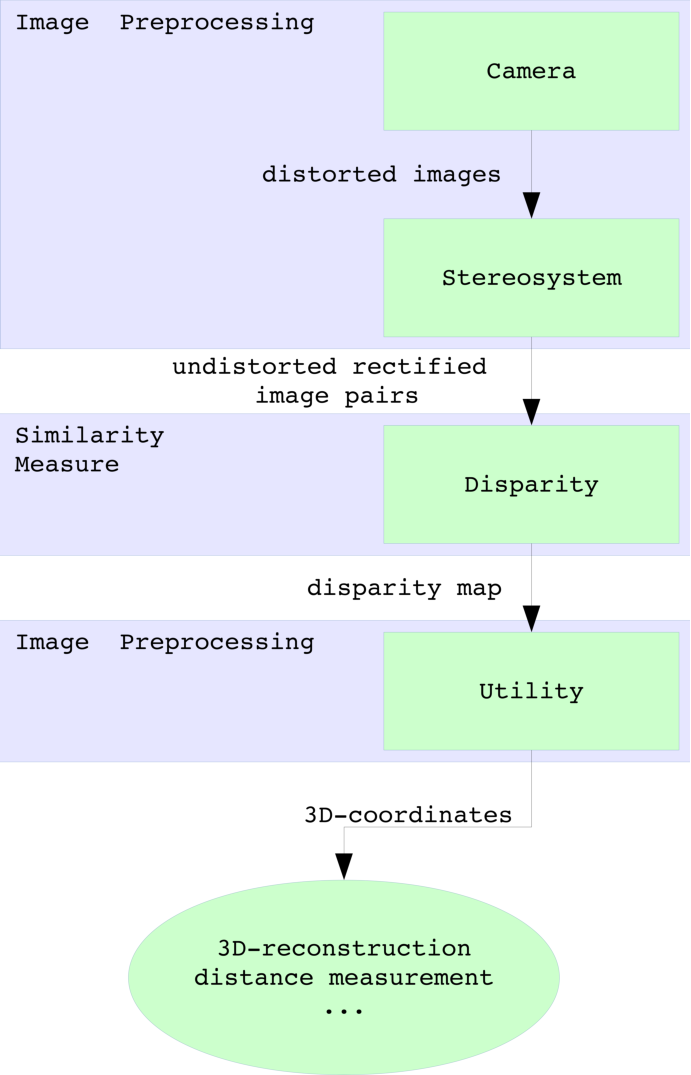
\includegraphics[width=0.5\textwidth]{images/graph_composition}
        \caption{Framework components}
        \label{fig:framework}
\end{figure}

The \texttt{Camera} class encapsulates the complete Matrix Vision API from the rest of the framework. On the one hand it realizes the image acquisition, on the other hand it allows to set some camera specific parameters like binning mode, exposure time or gain.

The images from the left and right cameras are then passed into the \texttt{Stereosystem} class. This class handles the complete stereo setup. It is responsible for calibration, undistortion and rectification. 

The \texttt{Stereosystem} class offers functions to calibrate the cameras with a given set of calibration images, save and load former calibration parameter and return different types of image pairs, namely distorted, undistorted and rectified image pairs.

After the \texttt{Stereosystem} class returns the rectified image pairs, they are passed to disparity calculations. At the moment the \texttt{disparity} namespace offers semi-global block matching, block matching and template matching for disparity calculation.

The generated disparity maps can then be used to calculate 3D coordinates. SInce this is just a single function (which is in fact just a single multiplication) we decided to put it into the \texttt{utility} namespace.

\bigskip
For several examples please have a look into the \texttt{example} directory or at the appendix. %TODO create examples


\section{Evaluation}
\section{Discussion}
\section{Future Work}

\nocite{*}
\bibliographystyle{acm}
\bibliography{reference}


\end{document}
